% popout, alpha = 2
\begin{figure}[H]
  \centering
	\begin{subfigure}{.7\textwidth}
    \centering
    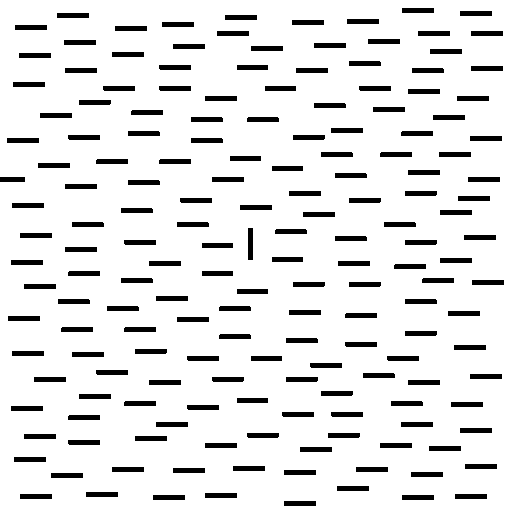
\includegraphics[width=.9\textwidth]{./canny/popout}
    \caption{Original popout image}
    \label{fig:popout}
  \end{subfigure}%    
  
    \begin{subfigure}{.7\textwidth}
    \centering
    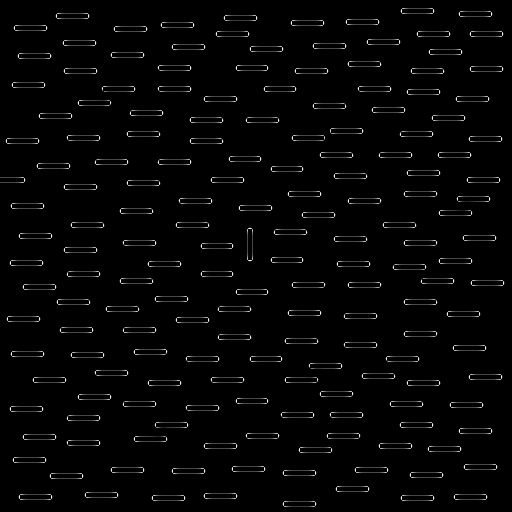
\includegraphics[width=.9\textwidth]{./canny/popout_LINF_a3_k11_k24}
    \caption{popout, Isotropic L-infinity norm. $\alpha$ = 3, K1 = 1, K2 = 4}
    \label{fig:popout_LINF_a3_k11_k24}
  \end{subfigure}%

\end{figure}

\begin{figure}[H]
\centering

  \begin{subfigure}{.7\textwidth}
    \centering
    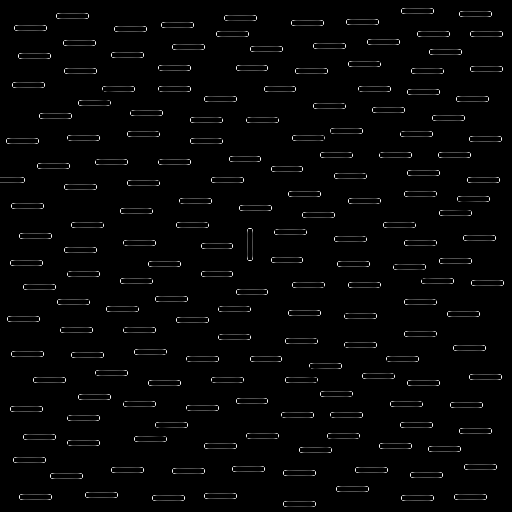
\includegraphics[width=.9\textwidth]{./canny/popout_L1_a3_k11_k24}
    \caption{popout, Isotropic L1 norm. $\alpha$ = 3, K1 = 1, K2 = 4}
    \label{fig:popout_L1_a3_k11_k24}
  \end{subfigure}%
  
  \begin{subfigure}{.7\textwidth}
    \centering
    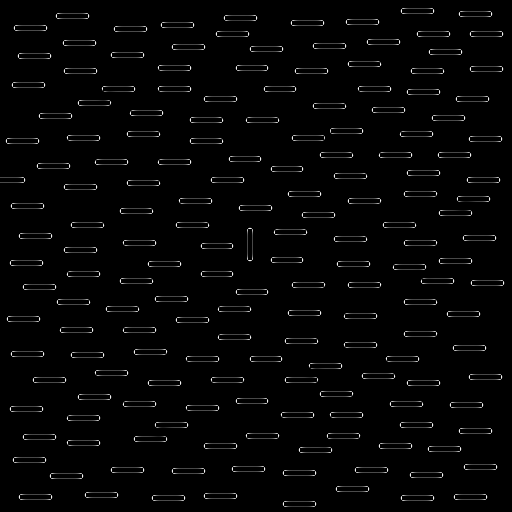
\includegraphics[width=.9\textwidth]{./canny/popout_L2_a3_k11_k24}
    \caption{popout, Isotropic L2 norm. $\alpha$ = 3, K1 = 1, K2 = 4}
    \label{fig:popout_L2_a3_k11_k24}
  \end{subfigure}\\%
 \end{figure}

\begin{figure}[H]
\centering 
  \begin{subfigure}{.7\textwidth}
    \centering
    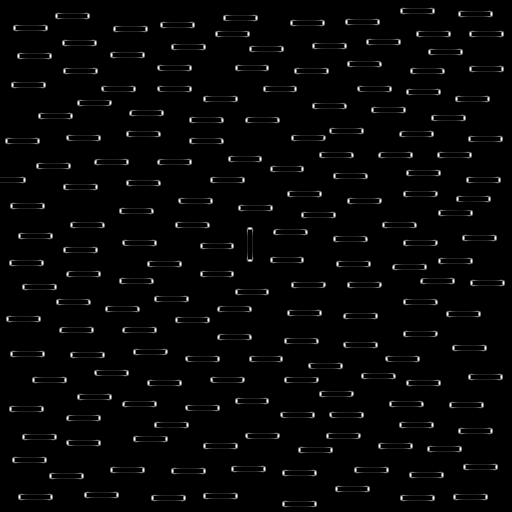
\includegraphics[width=.9\textwidth]{./canny/popout_ANISO_a3_k11_k24}
    \caption{popout, Anisotropic. $\alpha$ = 3, K1 = 1, K2 = 4}
    \label{fig:popout_ANISO_a3_k11_k24}
  \end{subfigure}%
  
\end{figure}